\section{The natural Wang rule and its proof}\label{sec:natural}

This section proves the dynamical equivalence on arbitrary raw Wang inputs. No result about token tables, machine simulation or a computed finite configuration is used. We first specify the rule, then prove one flag-only contour estimate. Two deterministic uses of that estimate finish the argument: coherence turns an old unmarked live region into a forbidden finite tiling, while a genuine tiling protects a live phase against the same marked field. All probabilities below concern independent update randomness; no averaging over tile sets is involved.

\subsection{Proof architecture}

There are three objects in the argument and two different uses of compactness. The deterministic rule reads tile letters. The random maps couple arbitrary starts. The marked field forgets the letters entirely and records only where a two-cluster explanation can end in flags. We prove estimates for that field before asking whether the tiles tile. This order makes the noise threshold independent of the input and prevents a hidden union over the input alphabet.

For a non-tiling input the logical certificate is finite: one square has no legal filling. Coherence first turns transverse comparisons into ordinary matching equations. Backward growth then produces a legal filling of that square from any sufficiently old unmarked live output. This deterministic contradiction places every late live output inside the marked field. Only at the last step do we compare two arbitrary starts: any discrepancy must contain a live letter in one of them and therefore follows a marked path. The path-tail estimate controls the event that \emph{some} pair could differ.

For a tiling input no forbidden square is available. Instead the tiling supplies a fixed reference configuration. A wrong output requires more failed providers than a single cluster can hold. Its error set is thus covered by the very same marked field. The blank reference has its own error cover. Sparse one-point marks, rather than a path-tail estimate, are enough to keep their one-site densities apart forever.

The first compactness use is logical: legal finite squares of all sizes would yield a plane tiling, so non-tiling has a finite witness. The second is probabilistic: Ces\`aro limits give stationary laws on a compact configuration space. Neither compactness argument asserts a computable bound on when a limit or certificate appears. The quantitative information comes separately from finite-age coherence and the finite-contour counting.

\begin{table}[ht]
\centering\small
\begin{tabularx}{\textwidth}{@{}>{\raggedright\arraybackslash}p{3.1cm}>{\raggedright\arraybackslash}X>{\raggedright\arraybackslash}X@{}}
\toprule
Ingredient & Non-tiling direction & Tiling direction\\
\midrule
Finite certificate or reference & forbidden $n_R$-square & a plane tiling $\theta$\\
Deterministic use of the quorum & coherence and backward growth & two-cluster error cover\\
Required flag estimate & tail of marked paths & probability of a marked root\\
Stationary conclusion & one law attracting all starts & two laws with a fixed density gap\\
Input-dependent quantity & delay $762n_R+1$ & reference letters only\\
\bottomrule
\end{tabularx}
\caption{The two uses of one marked field. The contour constants and the permitted noise interval are the same in both columns.}
\end{table}
\subsection{Tiles, configurations and noise}

A Wang tile is an oriented unit square with four named edge colours. A finite Wang set $R$ tiles the plane if there is $\theta:\Z^2\to R$ whose shared horizontal and vertical edge colours match. Translations are allowed, rotations and reflections are not. The tiling space $\nwT(R)$ is the closed subset of $R^{\Z^2}$ given by these matching equations. A finite legal pattern need only match its internal edges; no extendibility beyond its domain is assumed. Keeping this distinction is essential: a non-tiling set can have very large legal finite patterns.

The alphabet is
\[
 A_R=R\sqcup\{\bot\},\qquad \Omega_R=A_R^{\Z^6}.
\]
The new symbol $\bot$ is blank; every other letter is \emph{live}. We write a spatial site as $v=(u,P)$, where $u\in\Z^2$ is planar and $P\in\Z^4$ is transverse. The product topology of discrete alphabets makes $\Omega_R$ compact and metrizable. A cylinder event reads finitely many sites; it is both open and closed. A probability measure is stationary if applying one update leaves it unchanged. Spatial translation invariance always means invariance under every translation of $\Z^6$, unless a smaller group is explicitly named.

Let
\[
 \Gamma=\{0,e_1,-e_1,e_2,-e_2\},\qquad
 \Lambda=\{-1,0,1\}^2.
\]
The cardinal checker $C_R$ applied in a planar layer retains the central tile precisely when all five letters at $u+\Gamma$ are live and the four shared edges at $u$ match. Otherwise it outputs $\bot$. A successful check therefore retains an \emph{original} tile of $R$. It introduces no bit, block presentation or auxiliary symbol.

Given a deterministic finite-range rule $G_R$, use independent variables
\[
 \eta_t(v)\sim\operatorname{Bernoulli}(\eps),\qquad
 \zeta_t(v)\sim\operatorname{Unif}(A_R)
\]
at every site and update time. The two fields are independent. From a start $x$ at time zero,
\begin{equation}\label{nw:update}
 X_t^x(v)=
 \begin{cases}
 \zeta_t(v),&\eta_t(v)=1,\\
 G_R(X_{t-1}^x)(v),&\eta_t(v)=0.
 \end{cases}
\end{equation}
Every start uses the same fields. An indicated replacement is charged as a possible error even when its value happens to be correct. For $m=|A_R|$ the stochastic table is
\begin{equation}\label{nw:table}
 p_{R,\eps}(a\mid y)=(1-\eps)\mathbf1_{\{a=G_R(y)\}}+\eps/m.
\end{equation}
Thus every entry is at least $\eps/m>0$. The operation replaces the whole symbol after the deterministic update.

\subsection{Five fixed provider boxes}

In the transverse lattice put
\begin{align}\label{nw:boxes}
 K&=16^4,& C_0&=0,& C_i&=160e_i\quad(1\le i\le4),\notag\\
 S_i&=C_i+\{0,\ldots,15\}^4,&S&=\bigcup_{i=0}^4 S_i,&q&=5K,\quad h=4K.
\end{align}
The boxes are disjoint. Each contains $K$ offsets, and $S$ contains $q$ offsets. We call the $S_i$ clusters. Set
\[
 y(u,Q)=C_R(x(\cdot,Q))(u).
\]
The clustered quorum is
\begin{equation}\label{nw:rule}
 G_R(x)(u,P)=
 \begin{cases}
 s,&s\in R,\quad|\{a\in S:y(u,P+a)=s\}|\ge h,\\
 \bot,&\text{if no such live }s\text{ exists}.
 \end{cases}
\end{equation}
Two distinct live letters cannot both qualify, since $2h=8K>5K=q$. Blank readings do not vote. All boundary equalities in this definition are intentional: exactly $h$ agreeing readings suffice.

The actual neighbourhood is $\Gamma\times S$. We also use the fixed enclosing neighbourhood
\begin{equation}\label{nw:neighbourhood}
 \overline N=\Lambda\times S.
\end{equation}
The latter contains zero; redundant inputs are ignored in \eqref{nw:rule}. The geometry is fixed before $R$: only the alphabet and its four matching tests vary. Exhaustive enumeration of parent words computes the finite table from $R$. Its size is very large but finite, which is all that computability requires.

For estimates put
\begin{equation}\label{nw:constants}
 \Delta=18q,\qquad B=2\Delta^2,\qquad
 \eps_*=B^{-200},\qquad\kappa=4B^{-99},\qquad
 c=\frac{\log(1/\kappa)}{50}.
\end{equation}
These are effective constants independent of $R$. Indeed $q=5\cdot2^{16}$, $\Delta=90\cdot2^{16}$ and $B=16200\cdot2^{32}>2^{45}$. In particular $\kappa<1$. Numerical sizes are orientation only; every estimate will follow from the displayed integer inequalities.

\subsection{The geometry behind the two budgets}

The boxes serve two jobs. Their separation supplies affine charges with positive drift away from one bad cluster per charge. Their thickness supplies many offset pairs one lattice step apart. Only the second job is used for coherence; only the first is used to count contours. A large separation cannot compensate for an overlap deficit, and a thick box alone cannot supply the balanced charge condition. The choices $16$ and $160$ meet both requirements with explicit slack.

The number $q$ counts provider offsets, not checker input sites. One provider reads five cardinal letters; nearby providers in the same transverse box lie in different planes. During the proof the enclosing Moore graph allows nine planar offsets per provider and hence $9q$ backward neighbours. We use its undirected degree $18q$ to count connected edge witnesses. This degree is deliberately an overestimate for the actual rule. It also lets the later robustness statement allow maps on every input of $\overline N$ without changing the path count.

\begin{figure}[ht]
\centering
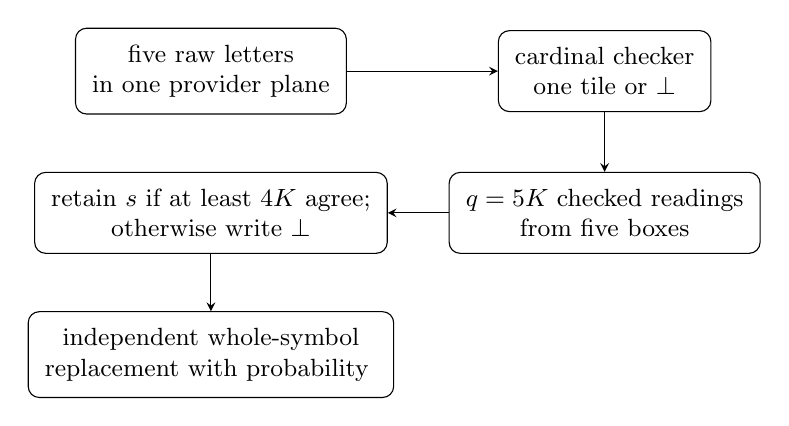
\begin{tikzpicture}[>=stealth,box/.style={draw,rounded corners,align=center,font=\small,inner sep=6pt}]
\node[box] (old) at (0,0) {five raw letters\\in one provider plane};
\node[box] (check) at (5.0,0) {cardinal checker\\one tile or $\bot$};
\draw[->] (old)--(check);
\node[box] (votes) at (5.0,-1.8) {$q=5K$ checked readings\\from five boxes};
\node[box] (out) at (0,-1.8) {retain $s$ if at least $4K$ agree;\\otherwise write $\bot$};
\draw[->] (check)--(votes);
\draw[->] (votes)--(out);
\node[box] (noise) at (0,-3.6) {independent whole-symbol\\replacement with probability $\eps$};
\draw[->] (out)--(noise);
\end{tikzpicture}
\caption{One local update. The checker is repeated once per provider offset. The noise is applied after the quorum and replaces the entire output letter.}
\end{figure}

A live output guarantees at least $h$ successful providers. Failure is therefore permitted at $q-h=K$ offsets. Independently of their letters, an unmarked root has affected inputs in at most one cluster, also $K$ offsets. Successful and unaffected providers can thus be found by discarding at most $2K$ offsets. When two roots are compared, injectivity of the offset pairing turns their two exclusion budgets into at most $4K$ lost pairs. This is why the within-box unit-shift count must exceed $4K$, rather than merely exceed the number of failed votes.

For memory the inequality is read in the opposite direction. To erase a correct reference tile, there must be $q-h+1=K+1$ failed providers. The extra one matters: $K$ failures would leave exactly the quorum of $4K$ correct votes. Since no one box has $K+1$ providers, those failures occupy two clusters and seed the mark recurrence. This explains the use of a nonstrict quorum threshold together with a strict failure count.
\subsection{Three elementary inputs}

The empty input needs no convention about a uniform law on an empty set: the actual alphabet is $A_\varnothing=\{\bot\}$, and replacement is uniform on this one-point alphabet. The checker, quorum and noisy process all have one possible output. This input is non-tiling and its dynamics is immediately ergodic. Separating it explicitly also avoids applying a later positive-table theorem whose standing assumptions require at least two letters.

Next let $R=\{r\}$ with its opposite edge colours matching. There is exactly one planar tiling, the constant $r$ tiling. Writing $b(u,P)=\mathbf1_{\{x(u,P)=r\}}$, the deterministic rule has the completely explicit binary form
\[
 G_R(b)(u,P)=\mathbf1\left\{
 \sum_{a\in S}\prod_{d\in\Gamma}b(u+d,P+a)\ge4K\right\}.
\]
A checked vote is one exactly when all five cardinal inputs are one. Uniform replacement writes zero and one with equal conditional probability at a flag. The two deterministic constant configurations are references for the two-cluster error cover. The theorem proves two distinct stationary laws for this noisy binary rule throughout the common interval. It makes no claim here that these exhaust the stationary laws or that the original unstacked rule has a continuum of extremes. That is precisely the countable-tiling case left open later.

Finally let $R=\{r\}$ but give $r$ different north and south colours. A live centre cannot pass both vertical matching tests, whatever its neighbours, since the only live neighbour letter is again $r$. Thus $C_R$ and $G_R$ are identically blank on every input configuration. Under uniform replacement, the next row is independent of the old row and has independent live indicators of probability $\eps/2$. It has a unique product stationary law, reached after one step. The general forbidden-square estimate is valid but far from sharp in this example: the first forbidden square only provides a convenient certificate for a proof that must also handle arbitrarily complicated inputs.

These examples illustrate what is held fixed in the family. The two singleton inputs have the same binary alphabet operation, the same boxes, the same quorum and the same noise rate. Only the tile's edge-matching test changes. On a general input the labels $r$ themselves are retained by a successful check, so one is still applying the same formula to raw tiles. There is no preliminary recognition of whether the input is one of these elementary examples, nor any conditional choice of a machine simulation. The finite table is generated uniformly by the checking prescription.

The mismatched singleton is also useful for the scope of robustness. Its base dynamics has no dependence on the past at all. Nevertheless a nearby table with an arbitrarily enlarged neighbourhood can read enough sites to recover a stable binary majority signal. The counterexample in \cref{nw:unrestricted} therefore cannot be dismissed as a perturbation of a finely tuned complicated input. What must be bounded in the robustness theorem is the specified input neighbourhood, not the logical difficulty of the tile set.
\subsection{The all-input coefficient and the theorem}

Each innovation $(\eta_t(v),\zeta_t(v))$ specifies a local map from parent words to output letters: either $G_R$ or a constant map. Composing these maps through a depth-$t$ cone at $v$ gives a random function of the initial row. Define
\begin{equation}\label{nw:qt}
 a_t=\Prob\{x\longmapsto X_t^x(v)\text{ is not constant on }\Omega_R\}.
\end{equation}
Translation covariance makes this probability independent of $v$. At a fixed finite time only finitely many initial sites can affect $v$. Thus constancy is a finite test for each innovation realization, and the event in \eqref{nw:qt} is measurable. The pair of starts witnessing nonconstancy may be chosen \emph{after} the innovations are known.

This is stronger than a bound for every fixed pair of starts. If a single noise event covers all possible discrepancies, it bounds $a_t$ without a union over starts. For a finite observation set $O$, a union over the output sites gives
\begin{equation}\label{nw:window}
 \Prob\{x\longmapsto X_t^x|_O\text{ is not constant}\}\le |O|a_t.
\end{equation}
The same estimate bounds the total-variation distance between the two $O$-marginals from any two initial laws, by common-map coupling. Independence of the chosen initial states from future innovations is sufficient.

\begin{theorem}[Natural Wang classification]\label{nw:classification}
For every finite Wang set $R$ and every $0<\eps\le\eps_*$, the rule \eqref{nw:rule} with uniform whole-symbol replacement is ergodic if and only if $R$ does not tile $\Z^2$. If $R$ tiles, there are two distinct spatially translation-invariant stationary laws. If $R$ has no legal $n\times n$ pattern, $n\ge1$, then for every $t\ge0$,
\begin{equation}\label{nw:coalescence}
 a_t\le \frac{1}{1-\kappa}\exp\{c(762n+1-t)\}.
\end{equation}
The constants $\eps_*,\kappa,c$ are the same for all $R$.
\end{theorem}

The proof occupies the rest of this section. Its contour, path and coherence arguments are the raw-letter forms of \cite[Lemmas~5.1--5.3]{DMdiagram}; the complete-history compactness argument below corresponds to that paper's Lemma~8.5. Lemma~5.4 there concerns deep wrong readings of an auxiliary forecast; that extra device is absent from the bare rule and is not required here. The quantitative finite-history method follows its Theorem~9.5 and Appendix~A, specifically Lemmas~A.1--A.2. Those results belong to the version~1.1.0 package directed by Nidhal Mghirbi. The finite certificate here is simply a forbidden square, which removes the statistical eraser and grouped rare-birth estimates needed there. The charge-arm method itself is due to Toom, Berman--Simon and G\'acs \cite{Toom80,BermanSimon88,Gacs21}.

\subsection{A marked field determined only by flags}

For now sample the Bernoulli flags at all integer times, including auxiliary negative times. An ordinary backward edge is
\begin{equation}\label{nw:edge}
 (u,P,t)\longrightarrow(u+d,P+a,t-1),
 \qquad d\in\Lambda,\ a\in S.
\end{equation}
The associated undirected graph has degree at most $2\cdot9q=\Delta$. Each edge changes time by exactly one. The larger Moore neighbourhood is convenient for estimates and robustness; the deterministic rule uses only its cardinal subset.

For an integer $t_0$, start a marked set empty at time $t_0$, and thereafter mark every flagged vertex and every vertex having marked parents in two distinct transverse clusters. The union as $t_0\to-\infty$ is denoted $\nwM$. Equivalently it is the least set containing all flags and closed under the rule
\begin{equation}\label{nw:mark}
 \begin{split}
 &(u+d,P+a,t-1)\in\nwM,\quad
 (u+d',P+a',t-1)\in\nwM,\\
 &a\in S_i,\ a'\in S_j,\ i\ne j
 \quad\Longrightarrow\quad (u,P,t)\in\nwM.
 \end{split}
\end{equation}
The closure is finitary: every marked point has a finite derivation from flags. Taking derivation depth as rank and selecting two lower-rank supports at each nonflagged mark yields a finite root-reachable acyclic support graph. Branches may merge. Its terminals are distinct physical flagged vertices, not independent copies of repeated appearances of one flag.

\paragraph{Least closure and finite supports.}
One can define the field without reference to a start time. Let $E$ be the set of flags, let $\Phi(J)$ add to $J$ every vertex with two distinct-cluster parents in $J$, and put $J_0=E$, $J_{r+1}=\Phi(J_r)$. Then $\bigcup_{r\ge0}J_r$ is closed: a supporting pair belongs to two finite ranks and therefore to their maximum rank. It is contained in every closed superset of $E$, so is the least one. This agrees with the increasing finite-start construction. A finite-rank derivation uses finitely many parents recursively and reaches a finite earliest time; starting empty before that time realizes the same mark. Conversely every finite-start mark has a finite-rank derivation by induction on elapsed time.

This equivalence distinguishes the least closure from any larger solution of the recurrence. For example, marking all vertices would satisfy the propagation implication but would not have finite flag witnesses. Every argument below concerns the least closure. The supports selected for a nonflagged marked vertex can be chosen at strictly smaller derivation ranks. Terminating at flags gives a finite graph, even though the full lattice and its past are infinite. If the same ancestor is reached by two branches it is retained once as a physical vertex. The graph can have undirected cycles, but no directed cycle, because each edge decreases time. These are exactly the properties used by the frontier construction.
\begin{lemma}[The unmarked exclusion budget]\label{nw:budget}
An unmarked vertex is unflagged. Among its provider offsets $a\in S$, at most $K$ have any marked Moore parent $(u+d,P+a,t-1)$, $d\in\Lambda$.
\end{lemma}
\begin{proof}
If marked parents occurred in two different clusters, \eqref{nw:mark} would mark the vertex. They therefore occur in at most one cluster, containing $K$ offsets. A flag is a mark by definition.
\end{proof}

This assertion depends on the flag field alone. It holds simultaneously for every trajectory and every choice of letters written at flags. In particular it remains valid for starts selected with knowledge of the noise; no causality assertion about such selected starts is needed for this deterministic step.

\subsection{Five balanced charges}

Ignore $u$ and assign the potentials
\begin{equation}\label{nw:potentials}
 \psi_0(P,t)=5\sum_{i=1}^4P_i+640t,\qquad
 \psi_i(P,t)=-5P_i-160t\quad(1\le i\le4).
\end{equation}
Their sum is identically zero. A backward edge with transverse displacement $a$ has gains $5\sum_i a_i-640$ for charge zero and $160-5a_i$ for charge $i$. If its cluster is nonzero, the first gain is at least $160$. If its cluster differs from $i$, the second gain is at least $160-75=85$. All gains, including the other choices, are at least $-715$.

For any two selected supports in distinct clusters, every charge can choose one of them with gain at least $85$: charge zero avoids cluster zero, and charge $i\ge1$ avoids cluster $i$. Call that support good for the charge. The choices for different charges can differ. A support graph is not a tree of five independent paths; the same physical edge or terminal may be used by several arms. The next construction keeps that multiplicity for the potential accounting and removes it only when counting physical witnesses.

\paragraph{Checking every gain analytically.}
For charge zero, offsets in $S_0$ have coordinate sum between zero and $60$, so the gain lies between $-640$ and $-340$. In any nonzero cluster that sum is between $160$ and $220$, giving gains between $160$ and $460$. For charge $i\ge1$, a provider in cluster $i$ has coordinate $a_i$ between $160$ and $175$, giving gains between $-715$ and $-640$. In any other cluster $a_i$ is between zero and $15$, giving gains between $85$ and $160$. These interval computations check all offsets at once. There is no enumeration of the $5\cdot16^4$ providers and no finite computed premise.

\begin{table}[ht]
\centering\small
\begin{tabular}{@{}lcc@{}}
\toprule
Charge & its excluded cluster & every other cluster\\
\midrule
$0$ & $[-640,-340]$ in $S_0$ & $[160,460]$\\
$i\in\{1,2,3,4\}$ & $[-715,-640]$ in $S_i$ & $[85,160]$\\
\bottomrule
\end{tabular}
\caption{Backward gains. A support pair in distinct clusters always includes a good choice for every charge. The sum of the five potentials is zero at every source and every terminal.}
\end{table}

The balance is algebraic, not a probabilistic cancellation. Each transverse coefficient $5P_i$ of $\psi_0$ cancels the coefficient $-5P_i$ of $\psi_i$, and $640t$ cancels four copies of $-160t$. The possible negative gain pays only for first edges introduced when a frontier component splits. That is why the edge bound is proportional to the number of \emph{new sources}, which is the number of distinct selected flags minus one. Counting all branch occurrences instead would lose the useful Bernoulli exponent.
\begin{lemma}[Finite charge-arm witness]\label{nw:arms}
For a marked root there is a connected physical ordinary-edge witness containing the root and $f\ge1$ distinct flags. It has an abstract copied-arm realization with at most
\begin{equation}\label{nw:armcount}
 e_{\rm arm}\le\frac{4000}{85}(f-1)<50(f-1)
 \quad\text{when }f>1
\end{equation}
edge occurrences. Its physical edge count and its time span are at most $e_{\rm arm}$. A flagged root may use the singleton witness $f=1$, $e_{\rm arm}=0$; an unflagged root has $f\ge2$.
\end{lemma}
\begin{proof}
Stop the finite support graph at flags. Name a terminal by its physical space--time coordinate, and for each vertex $v$ let $D(v)$ be its nonempty set of descendant terminal names. At a nonterminal with selected supports $a,b$,
\[
 D(v)=D(a)\cup D(b).
\]
We first construct arms so that distinct terminal names, rather than unfolded tree leaves, pay for their length.

Expose the graph from root to terminals in a topological order. A frontier is the set of unexposed vertices currently reached. Join two frontier vertices when their descendant terminal sets overlap. Initially the frontier is just the root. Exposing $v$ replaces it by its supports, retaining one physical copy of an already present support. Because $D(a)$ and $D(b)$ are subsets of $D(v)$, the replacement cannot meet an outside overlap component. It splits its own component into at most two. To verify the latter assertion, follow an old overlap path from a remaining vertex toward $v$. Its last common terminal with $v$ belongs to $D(a)$ or $D(b)$, so its remaining part attaches to one of the supports. Every resulting component therefore contains $a$ or $b$. In a genuine split the two daughter components have disjoint sets of descendant terminal names.

Fix a good-parent choice for every charge at every nonterminal. Starting at a given support and repeatedly following good parents reaches a terminal, since the support graph is finite and acyclic. Begin with one source occurrence at the root and five good arms, one for each charge. Track each arm by its eventual terminal name. Maintain the invariant that in each frontier overlap component there is exactly one endpoint name for each charge, counting arm occurrences.

When exposure causes no split, the invariant persists: a terminal name in the old component still lies in its one successor component. At a split at $v$, the existing endpoint for each charge belongs to exactly one daughter. Add one new source occurrence at $v$. For that charge choose the support in the daughter missing its old endpoint, take this first edge, and then follow good parents to a terminal there. The first edge need not be good; every later edge is good. Do this for the five charges. The new source restores one endpoint of each charge in each daughter. If the split is at the original root, keep the new source occurrence distinct from the original one even though their physical coordinates coincide.

At the final frontier each component is one terminal name. For each charge, source occurrences and terminal names are in bijection via their arms. Now take separate abstract copies of all arm interiors. Identify the five starts belonging to a source occurrence, and identify endpoints with the same terminal name. Keep different source occurrences distinct even when their coordinates agree. Retain the connected component containing the original root source. Restricting the charge bijections to it is valid, since every arm connects its source and endpoint within a single component. If $f$ terminal names remain, exactly $f$ source occurrences remain, with one incidence of each charge at each source and terminal.

At most $5(f-1)$ edges are bad: only the first edge from each nonoriginal source can be bad for its charge. Sum potential increments along all abstract arms, with their multiplicities. At each source the sum of the five starting potentials is zero; at each terminal the sum of the five ending potentials is zero. Thus the total increment equals zero. Every good edge gains at least $85$, every bad edge at least $-715$. Consequently
\[
 0\ge85e_{\rm arm}-(85+715)5(f-1),
\]
which gives \eqref{nw:armcount}. An unflagged original source has outgoing good edges, so $e_{\rm arm}>0$ and $f\ge2$.

Projection of the retained abstract component to physical edges is connected, contains the root and the $f$ distinct flags, and can only reduce the edge count. Every projected vertex is at or before the root time. A vertex of minimum time in the abstract graph must be a terminal: a source or arm interior has an outgoing edge to an earlier time. A simple undirected path in this connected graph from the root to a minimum-time terminal uses at most $e_{\rm arm}$ edge occurrences. Each changes time by exactly one, so its time span is at most $e_{\rm arm}$. Every vertex lies between those two times. No unary edge or identification changes the clock, because there are no unary links and terminal names are actual space--time coordinates.
\end{proof}

The separation of abstract arms from physical edges is load-bearing. Potential telescoping uses one arm of each charge per terminal, whereas probability uses one Bernoulli factor per \emph{distinct} flag. Unfolding a merged support graph into a tree and counting its leaves as independent would not justify the bound.

\paragraph{What a split preserves.}
The frontier is a partition of the remaining terminal names into overlap components, rather than a partition of the original support vertices into independent branches. After exposing a vertex, all terminal names previously reachable are still reachable through one of its supports. If the component splits, its two terminal-name unions are disjoint. Each old arm endpoint therefore has one definite daughter, even if several abstract arms pass through the same physical intermediate vertex. Adding a new source supplies only the missing daughter for each charge; it does not duplicate an already counted flag.

At the end a source-to-terminal arm graph may have several connected components. Discarding those away from the original root is legitimate for two reasons. First, every retained arm connects one retained source to one retained terminal, so each charge's bijection restricts to the retained component. Second, the potential sum is balanced at each individual source and terminal, so it telescopes within that component without using discarded arms. This is why the proof can obtain a connected physical witness and an exact count of distinct terminal flags at the same time. Neither connectedness nor distinctness is inferred from the support graph being a tree.
\subsection{Counting connected witnesses}

Fix an ordering of the at most $\Delta$ neighbours of every vertex of the ordinary graph. A connected $n$-edge set containing a specified root can be doubled to an Eulerian multigraph. Choose a deterministic Euler walk starting at that root. Its $2n$ neighbour indices encode the edge set, so there are at most $\Delta^{2n}$ possible sets. The walk may revisit vertices and edges; that is why doubling suffices even when the physical witness has cycles.

A connected $n$-edge set has at most $n+1$ vertices. At most $2^{n+1}$ subsets can be designated as terminal flags. We may count every subset, including impossible support witnesses, since this is an upper bound. Combining the counts gives
\begin{equation}\label{nw:encoding}
 \#\{\text{rooted edge set, terminal subset}\}
 \le2(2\Delta^2)^n=2B^n.
\end{equation}
For a fixed subset of $f$ distinct vertices, the probability that all are flags is exactly $\eps^f$. The remaining support conditions are discarded. Thus adaptive selection of a support graph never creates a conditional independence claim: we take a countable union over deterministic finite witnesses.

\begin{lemma}[Sparse roots]\label{nw:sparse}
At every vertex, uniformly in $R$ and $0<\eps\le\eps_*$,
\begin{equation}\label{nw:rootbound}
 \Prob(v\in\nwM)\le
 \eps\left(1+\frac{2\lambda}{1-\lambda}\right)<2\eps,
 \qquad\lambda=B\eps^{1/50}.
\end{equation}
The same strict bound holds with a source density $e\le2\eps_*$ in place of $\eps$.
\end{lemma}
\begin{proof}
A flagged root costs $\eps$. Otherwise its witness has $n\ge1$ physical edges and $f\ge1+n/50$ distinct flags, by \cref{nw:arms}. For a fixed terminal subset this costs at most $\eps^{1+n/50}$. Therefore \eqref{nw:encoding} gives
\[
 \Prob(v\in\nwM)\le\eps+
 \sum_{n\ge1}2B^n\eps^{1+n/50}
 =\eps\left(1+\frac{2\lambda}{1-\lambda}\right).
\]
Since $\lambda\le B^{-3}\le1/8$, the bracket is less than $2$. For $e\le2B^{-200}$, $Be^{1/50}\le2^{1/50}B^{-3}<1/8$, using $B>2^{45}$. The identical argument applies.
\end{proof}

The estimate does not mention the alphabet size, the replacement values, or a property of $R$. It controls one binary field for all starts and all tile sets at once. A sparse one-point field alone does not exclude an infinite path; the following packing argument supplies that additional fact and its finite-prefix tail.

\subsection{Packing contours along a marked path}

\begin{lemma}[Finite marked-path tail]\label{nw:paths}
For a specified root and $N\ge1$, the probability of an ordinary backward path of $N$ edges all of whose vertices belong to $\nwM$ is at most
\begin{equation}\label{nw:pathtail}
 \sum_{f\ge\lceil N/50\rceil}(4B^{101}\eps)^f.
\end{equation}
Almost surely there is no infinite such path, simultaneously at every root. The finite bound holds for any independent source density $e$ after replacing $\eps$ by $e$.
\end{lemma}
\begin{proof}
Fix a finite marked path whenever one exists. At its root choose the full witness of \cref{nw:arms}, including its selected flags. If the earliest terminal has time $s$, restart at the path vertex at time $s-1$, provided the path has not ended. Repeat. Successive witnesses lie in disjoint closed time slabs, so all selected terminal flags are distinct across witnesses. This conclusion uses the span assertion, not just an edge count.

For one witness with $f_i$ flags, its span is at most $50(f_i-1)$. It covers at most that span plus one path steps, including the restart edge, hence at most $50f_i$. For the final witness retain the \emph{whole contour}, even if its earliest terminal is earlier than the path endpoint. Truncate only the connecting path piece. This preserves distinct terminals and gives the same upper bound on covered path length. In particular the total number $f=\sum_i f_i$ satisfies $N\le50f$.

The physical union of these witnesses and the used path pieces is connected and contains the original root and all $f$ selected flags. Each contour has at most $50(f_i-1)$ physical edges, and its connecting path piece at most $50f_i$ edges. Thus the union has at most $100f$ edges, and the convenient larger bound $101f$ is valid. A flagged path root is allowed: its singleton contour has zero edges and covers one restart step. This includes the case in which every path vertex is flagged.

For fixed $f$, sum the encoding bound over physical edge counts $0\le n\le101f$. The singleton case is included by allowing $n=0$ and overcounting its possible subsets. As $B\ge2$,
\[
 \sum_{n=0}^{101f}2B^n\le4B^{101f}
 \le(4B^{101})^f.
\]
Not every encoded subset has $f$ elements; count only those that do, bounded by the same expression. Their joint flag probability is $\eps^f$. A union over $f\ge\lceil N/50\rceil$ gives \eqref{nw:pathtail}. No path is counted independently of its contour: the connected witness already encodes the necessary union.

At the stipulated rate the base obeys
\[
 4B^{101}\eps\le4B^{-99}=\kappa<1.
\]
The tail tends to zero as $N\to\infty$. An infinite marked path gives a finite marked path of every length from its root; these events decrease. Their probabilities tending to zero suffices. Countably many roots give the simultaneous almost-sure statement. For source density $e$ the same proof uses $e^f$ for a fixed terminal subset.
\end{proof}

\paragraph{A ledger for the path witness.}
It helps to separate three counts. The number $f_i$ is the number of distinct flags selected by one contour, $e_i$ is its abstract arm length, and $n_i$ is the number of physical edges after projection. Their relations are $n_i\le e_i\le50(f_i-1)$ and span at most $e_i$. The connecting path portion is counted separately. It may cross edges of a contour already present in the union; charging it again only increases the upper bound. Successive contours can have geometric projections that meet, but their selected physical time slabs are disjoint, so their terminal flags remain distinct. Spatial overlap never changes their independent Bernoulli cost.

There is also a reason for keeping the last contour whole. If one cut that contour at the prescribed path endpoint, the newly exposed cut vertices would not necessarily be flags. They could not be charged with independent source probabilities. The complete final contour retains its genuine terminals, even when its bottom time is below the path endpoint. The only truncated object is the path connector, which can only shorten the edge count. Thus the lower bound $f\ge\lceil N/50\rceil$ and upper bound of $101f$ witness edges concern the same legitimate terminal subset.

The estimates are deliberately coarse. The exact arm coefficient is $4000/85=800/17<48$, whereas the path packing uses $50$ for span coverage and $101$ for its combined edge budget. The noise exponent $200$ leaves room beyond the resulting $101$ in the witness count. At the maximum permitted source density for the unperturbed rule the final geometric base is $4B^{-99}$. For robustness its source density merely doubles and the base becomes $8B^{-99}$, still below one. None of these margins depends on how late the first forbidden square appears.
\subsection{Successful and unaffected providers}

We turn from probability to deterministic geometry. Fix any flag realization, any replacement values and one arbitrary trajectory started at time zero. All coherence statements refer to that one trajectory; starts will be compared only after the deterministic statements are established.

An unmarked live output of age $t\ge1$ is an ordinary $G_R$ output, say $s$. Its successful-provider set contains at least $h$ offsets returning $s$. At most $q-h=K$ offsets fail. By \cref{nw:budget}, at most $K$ offsets have any marked Moore input. Call a provider \emph{good} if it is successful and unaffected by marked inputs. At least $h-K=3K$ providers are good. A good provider supplies five unmarked live cardinal inputs one time earlier, with central letter $s$ and matched central edges.

There are two different budgets here. For a single root we exclude at most $2K$ offsets to find good providers. To compare two roots through an injective pairing, we exclude at most $4K$ pairs. A provider can be affected even when its own central input is unmarked: all Moore inputs are charged so the exclusion is valid for every checker input. This conservative choice will also cover arbitrary maps on the enclosing neighbourhood in \cref{nw:robust}.

\subsection{Same-site coherence at finite age}

\begin{lemma}[Equality at one planar site]\label{nw:same}
In one trajectory started at time zero, two unmarked live readings at $(u,P,t)$ and $(u,Q,t)$ have the same tile whenever
\[
 d=\|Q-P\|_1\le t.
\]
\end{lemma}
\begin{proof}
Induct on $d$, uniformly over the time and planar site. If $d=0$, both readings are at the same physical vertex. For $d>0$, choose a coordinate $j$ on which $Q-P$ is nonzero, and let $\sigma$ be its sign. Pair offsets inside each box by
\[
 a\longleftrightarrow a'=a-\sigma e_j,
 \qquad a,a'\in S_i.
\]
For each cluster there are $15\cdot16^3$ pairs. Both coordinate projections of the pairing are injective. The total count is
\[
 5\cdot15\cdot16^3=\frac{75}{16}K.
\]
Each root excludes at most $K$ failed and at most $K$ affected offsets. Injectivity means these exclusions remove at most $4K$ pairs altogether, even if all exclusion sets are disjoint. There remain at least
\begin{equation}\label{nw:surplus}
 \left(\frac{75}{16}-4\right)K=\frac{11}{16}K>0
\end{equation}
pairs. Select one. Its central parents at $(u,P+a,t-1)$ and $(u,Q+a',t-1)$ are unmarked and live and retain the two respective root letters. Their transverse distance is exactly $d-1$, because the displacement on coordinate $j$ has moved one step toward zero and the other coordinates are unchanged. Also $t-1\ge d-1$. The induction hypothesis identifies the parent letters, hence the root letters.
\end{proof}

The induction is on transverse span, not on the number of initial configurations. It never assumes that different planes agree at age zero. Finite age is the resource that pays for finite span. In a complete trajectory the same finite induction works at every span because an arbitrarily long finite past is available.

\paragraph{Why the reduction of span is exact.}
Write $Q-P=(d_1,\ldots,d_4)$ and choose $j$ with $d_j\ne0$. With $\sigma=\operatorname{sign}(d_j)$ and $a'=a-\sigma e_j$, the parent displacement is $(Q+a')-(P+a)=(Q-P)-\sigma e_j$. Its $j$th absolute coordinate drops by one and its other coordinates do not change. Thus its $\ell^1$ norm is exactly $\|Q-P\|_1-1$ for either sign, including $|d_j|=1$. Pairing is not restricted by the size of $Q-P$: only the relative unit shift of the offsets must remain inside the box. Hence the same overlap surplus works for arbitrarily distant root planes, one induction step at a time.

Within one box, fifteen choices remain in the shifted coordinate and sixteen in each other coordinate. If $\sigma=1$, omit the face with local coordinate zero on the first side; if $\sigma=-1$, omit the face with local coordinate fifteen. The pairing is one-to-one in both directions. A discarded offset on either root side can therefore destroy at most one candidate pair. No independence or favourable correlation of the two roots' bad-provider sets is assumed. The inequality survives their worst-case placement.

This pairing also explains why comparing roots by directly intersecting their absolute provider locations is unnecessary. Distant translates of $S$ can be disjoint. The proof compares the \emph{relative} offsets $a,a'$ and uses the previous-age coherence assertion at the resulting parent span. What persists across the induction is the root letter: a successful check retains its central parent's raw tile, so the two letters being compared are carried unchanged into the induction hypothesis.
\subsection{Cardinal compatibility at finite age}

\begin{lemma}[Neighbouring planar readings]\label{nw:neighbours}
Let $\gamma\in\{\pm e_1,\pm e_2\}$. Unmarked live readings at $(u,P,t)$ and $(u+\gamma,Q,t)$ have matching shared edges if
\[
 t\ge\|Q-P\|_1+1.
\]
\end{lemma}
\begin{proof}
Again induct on $d=\|Q-P\|_1$. When $d=0$, both ages are positive. Their successful-provider sets each have size at least $h$, so they overlap in at least
\[
 2h-q=3K>0
\]
offsets. At a common offset $a$, the check at $u$ retains the first root tile $s$, and the check at $u+\gamma$ retains the second tile $s'$. Their old central sites are adjacent in the same provider plane. The first check certifies the matching edge between those two actual old letters; the second identifies the neighbour letter as $s'$. Thus the two retained tiles match. Unmarkedness of those old inputs is not needed in this base case.

For $d>0$ use the same injective unit-shift pairing as in \cref{nw:same}. Its surplus \eqref{nw:surplus} supplies a good provider for each root. Their central parents are unmarked, live and cardinal-adjacent in the planar coordinate, carry the root letters, and have transverse span $d-1$. Their age satisfies $t-1\ge d=(d-1)+1$. The induction hypothesis certifies their shared edge and hence the root edge.
\end{proof}

The extra unit of age in this lemma is necessary for the proof: at equal transverse coordinates, arbitrary initial adjacent tiles need not match. Equality at the same planar site has a tautological age-zero base, whereas compatibility first uses an actual checker update.

\subsection{Finite certificates of non-tiling}

\begin{lemma}[Forbidden square]\label{nw:forbidden}
If a finite Wang set $R$ does not tile the plane, there is $n_R\ge1$ for which no legal $n_R\times n_R$ pattern exists. A finite search for such an $n_R$ terminates exactly on non-tiling inputs.
\end{lemma}
\begin{proof}
For each $n$ enumerate all maps from $\{0,\ldots,n-1\}^2$ to $R$ and test the internal shared edges. This is finite. If the test has no survivor, a full tiling is impossible. Conversely, suppose patterns exist for every $n$. Taking patterns on centered squares of arbitrarily large odd side, extend each outside its square arbitrarily to a configuration in $R^{\Z^2}$; when $R$ is nonempty this is possible. A subsequence stabilizes successively on each centered square by finite pigeonhole and diagonal selection. Its limiting configuration matches every edge, since that edge lies in all sufficiently large squares. This is a tiling. For $R=\varnothing$ the first test is already empty. The contrapositive proves termination on every non-tiler.
\end{proof}

The search is a semidecision. On a tiling input it never finds an empty square. It supplies no total computable upper bound for the first empty square as a function of the finite input. The proof of forgetting may use that finite certificate without computing it uniformly on all inputs.

The relevant transverse diameter is
\begin{equation}\label{nw:diameter}
 D=\operatorname{diam}_{\ell^1}(S)=380.
\end{equation}
For two distinct nonzero cluster centres the distance is $320$; for cluster zero and a nonzero cluster it is $160$. Box corners contribute at most $4\cdot15=60$. Equality $380$ is attained, for example by taking the two centres $160e_1,160e_2$ with opposite allowable corners in every coordinate. A sum of $r$ provider offsets therefore has pairwise $\ell^1$ spread at most $Dr$: pair the corresponding summands in two sums and apply the triangle inequality. This statement concerns the $r$-fold sumset $S+\cdots+S$, not the dilation $\{ra:a\in S\}$.

\subsection{Deterministic mortality outside the marked field}

\begin{lemma}[Forbidden-square delay]\label{nw:mortality}
Suppose $R$ has no legal $n\times n$ pattern. Put
\begin{equation}\label{nw:delay}
 r=2n,\qquad T_R=(D+1)r+1=762n+1.
\end{equation}
For every realization of flags and replacement values, for every initial configuration and every $t\ge T_R$, every live output at age $t$ lies in $\nwM$.
\end{lemma}
\begin{proof}
Assume instead that an unmarked live reading occurs at $(u_0,P_0,t)$. At every unmarked live positive-time output, a good provider exists because $h-K=3K>0$. It supplies unmarked live cardinal inputs at all five sites one step earlier. Repeat this construction for $r$ steps. For each $w\in\Z^2$ with $\|w\|_1\le r$, choose a cardinal path of exactly $r$ planar steps from $u_0$ to $u_0+w$, padding a shorter path by zero steps. Following good providers along it produces an unmarked live reading at
\[
 (u_0+w,Q_w,t-r),\qquad
 Q_w\in P_0+\underbrace{S+\cdots+S}_{r\ \mathrm{summands}}.
\]
Different paths need not use the same providers or produce the same $Q_w$. Choose one reading for each $w$ in the ball. Any pair of these transverse coordinates is within $Dr$. Their common age obeys
\[
 t-r\ge Dr+1.
\]
The same-site lemma makes any alternative chosen reading at a planar site agree, and \cref{nw:neighbours} makes every internal cardinal edge of the ball match. Hence the selected raw letters form a legal pattern on that whole planar ball. The ball of radius $2n$ contains $[-n,n]^2$, and thus contains an $n\times n$ square. Restricting gives the forbidden pattern, a contradiction.

All uses of the update occur at positive ages, since $t-r\ge1$. No stationary law, statistical erasure event, or probability estimate has entered. Thus the contradiction holds for every noise realization and every start simultaneously.
\end{proof}

The factor $762$ is only a convenient explicit choice: $2n$ planar growth steps times transverse diameter plus age cost, followed by one checker step. It is not a sharp extinction horizon. Its significance is that the certificate changes the delay, while all contour constants were fixed before the certificate and before $R$.

\subsection{Age, span and planar growth in one picture}

The coherence induction spends one unit of age to remove one unit of transverse $\ell^1$ span. The backward-growth argument spends $r$ units of age to cover a planar ball, but can spread the transverse coordinate by as much as $Dr$. These are different costs. After growth, the readings to be compared all lie on the same old time slice. That slice must still have enough age for the neighbour lemma. The budget is therefore $t-r\ge Dr+1$, exactly the condition $t\ge(D+1)r+1$ used above.

\begin{figure}[ht]
\centering
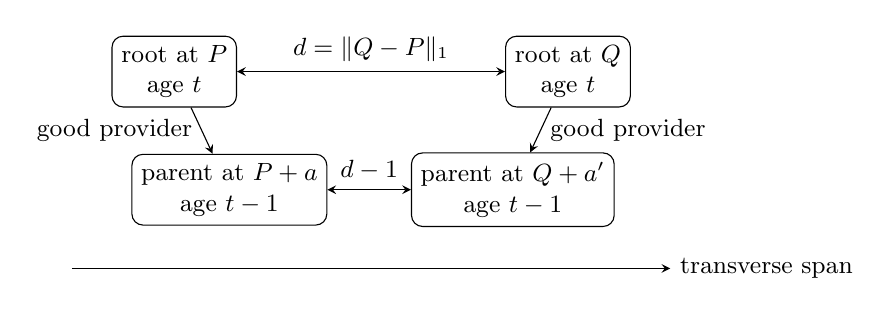
\begin{tikzpicture}[>=stealth,font=\small]
\draw[->] (-3.8,0)--(3.8,0) node[right]{transverse span};
\node[draw,rounded corners,align=center] (a) at (-2.5,2.5) {root at $P$\\age $t$};
\node[draw,rounded corners,align=center] (b) at (2.5,2.5) {root at $Q$\\age $t$};
\node[draw,rounded corners,align=center] (c) at (-1.8,1.0) {parent at $P+a$\\age $t-1$};
\node[draw,rounded corners,align=center] (d) at (1.8,1.0) {parent at $Q+a'$\\age $t-1$};
\draw[->] (a)--node[left]{good provider}(c);
\draw[->] (b)--node[right]{good provider}(d);
\draw[<->] (a)--node[above]{$d=\|Q-P\|_1$}(b);
\draw[<->] (c)--node[above]{$d-1$}(d);
\end{tikzpicture}
\caption{One coherence step, drawn schematically. The raw labels are retained along both arrows. Paired offsets $a'=a-\sigma e_j$ reduce the span while both ages drop by one. Absolute parent locations need not lie between the roots; only the relative span is depicted.}
\end{figure}

For the growth step, every planar displacement in the radius-$r$ ball is a sum of exactly $r$ members of $\Gamma$ because zero is allowed. This permits all supplied readings to be placed at the same past time. If one used only shortest paths, their ages would differ, and the stated coherence lemmas would not directly compare them. Padding by zero steps is the small but essential device that puts them on one common time slice.

Transverse readings at that slice lie in a sumset, because at every step a possibly different provider is chosen. The choices may depend on the trajectory and on the branch. Pairwise separation is nevertheless at most $Dr$, by matching the $r$ summands in any two selected paths. There is no requirement that one provider be good for all branches or that the whole grown patch lie in one transverse plane. Finite-age coherence supplies exactly the matching needed after the branchwise choices have been made.
\subsection{Tracing all possible discrepancies at once}

\begin{lemma}[All-input coalescence]\label{nw:allinput}
Under the hypothesis of \cref{nw:mortality}, \eqref{nw:coalescence} holds for all $t\ge0$. The bound is uniform over $0<\eps\le\eps_*$ and over all replacement-value laws that are independent of the configuration and shared across starts.
\end{lemma}
\begin{proof}
Fix the entire innovation realization. If the output map at $(v,t)$ is nonconstant, choose starts $x,x'$ for which the outputs differ. A discrepant positive-time vertex is not flagged, since a common replacement is constant in the parent word and writes the same value in both trajectories. Different deterministic outputs require a difference at some actual parent in $\Gamma\times S\subset\overline N$. Select such a parent and repeat.

At every discrepant vertex of age at least $T_R$, at least one of its two letters is live: two different letters cannot both equal $\bot$. By \cref{nw:mortality} that vertex belongs to the single field $\nwM$. Consequently, for $t>T_R$, existence of \emph{any} discrepant pair forces an ordinary marked backward path of $N=t-T_R$ edges from $(v,t)$ down to age $T_R$. This is a deterministic inclusion of events. Although the pair was chosen after seeing the innovations, its existence is covered by the same flag-only event; no sum over pairs or initial configurations is taken.

By \cref{nw:paths} and \eqref{nw:constants},
\begin{align*}
 a_t&\le\sum_{f\ge\lceil(t-T_R)/50\rceil}\kappa^f\\
 &\le\frac{1}{1-\kappa}
       \exp\left\{-\frac{\log(1/\kappa)}{50}(t-T_R)\right\}.
\end{align*}
For $t\le T_R$ the same bound is at least one, so $a_t\le1$ completes the estimate for all ages. The auxiliary negative-time flags caused no change to the positive-time process: the deterministic inclusion holds for every extension of its positive-time flags, so averaging over an independent extension is legitimate. Replacement values never enter the tail calculation.
\end{proof}

An event concerning only the number of bad letters for a chosen start would be insufficient here. The mortality statement is already universal over starts, and the marked-path event contains every discrepancy that could occur. This order of quantifiers is what later allows the all-DLR Gibbs theorem to be applied. The alphabet size creates neither a count of candidate trajectories nor a multiplicative factor in the rate.

\paragraph{Finite dependence and the order of quantifiers.}
For a fixed output vertex and a fixed time $t$, every initial site read by the composite lies in the $t$-fold sumset of the finite neighbourhood. There are finitely many such sites and finitely many initial words on them. Thus a pair witnessing nonconstancy can be selected from a finite set, without any measurable-selection issue. The proof does not sum the probabilities for those pairs. Instead it shows pointwise in the innovation realization that each possible discrepancy, whichever pair witnesses it, produces a path in the same pre-existing marked field.

The resulting probability statement is therefore $\Prob(\exists x,x':X_t^x(v)\ne X_t^{x'}(v))$, rather than merely $\sup_{x,x'}\Prob(X_t^x(v)\ne X_t^{x'}(v))$. The former bounds the latter but need not equal it for a general random-map representation. The stronger event gives a finite set of common maps on which every input row has the same output. This is the hypothesis used by the space--time transfer, and it is also the natural analogue of the retained all-input statement \cref{fgt:coalesce}, the strengthened form of Theorem~B(ii).

No initial word contributes a factor to the contour count. Even a start depending on the entire noise realization is covered by the pointwise inclusion, although attraction of an initial probability law is subsequently proved with an ordinary independent initial row. This distinction prevents any assumption that an adversarial choice of a witness pair remains independent of the marks. Only the fixed terminal subsets in the witness union require independence, and they consist of distinct Bernoulli flag variables.
\subsection{From common maps to ergodicity}

\begin{lemma}[Stationary existence and all-law attraction]\label{nw:ergodic}
A finite-range finite-alphabet PCA is Feller and has a stationary probability measure. If its all-input coefficient tends to zero, its stationary measure is unique and attracts every initial law. In the present non-tiling case, for its stationary law $\pi_R$ and every finite $O$,
\begin{equation}\label{nw:attraction}
 \sup_{\lambda}\dtv((\lambda P_{R,\eps}^t)_O,(\pi_R)_O)
 \le |O|\frac{e^{c(T_R-t)}}{1-\kappa}.
\end{equation}
\end{lemma}
\begin{proof}
The expectation of a cylinder function after one step depends on finitely many old coordinates and is continuous. Cylinder functions uniformly approximate continuous functions on the compact product space, so the transition operator preserves continuity. Thus it is Feller.

For any initial law $\lambda$, its Ces\`aro means
\[
 \nu_N=\frac1N\sum_{s=0}^{N-1}\lambda P^s
\]
have a weakly convergent subsequence by compactness of probability measures on a compact metrizable space. For a bounded continuous $f$,
\[
 (\nu_NP-\nu_N)(f)=\frac{(\lambda P^N)(f)-\lambda(f)}N
 \longrightarrow0.
\]
The Feller property passes this identity to a weak limit, which is stationary.

Choose a row of that stationary law $\pi_R$ and a row of an arbitrary law $\lambda$, independently of future innovations, and evolve both by the common maps. On any realization where the time-$t$ map is constant on $O$, the two output words agree. Their total-variation distance is bounded by $|O|a_t$ through \eqref{nw:window}. This tends to zero and gives \eqref{nw:attraction}. Replacing $\lambda$ by another stationary law shows equality of its every finite marginal with $\pi_R$, hence equality of the laws. Convergence of all finite marginals implies weak convergence: uniformly approximate a bounded continuous function by a cylinder function and then use finite-marginal convergence. No spatial invariance of $\lambda$ is assumed.
\end{proof}

If $R=\varnothing$, $A_R$ is a singleton and there is only one configuration. All assertions in the non-tiling direction are then immediate. It is harmless to apply the elementary lemmas above to that case, but later theorems stated for alphabets of at least two symbols will instead treat it separately.

\subsection{A tiling protects two reference phases}

Let $\theta\in\nwT(R)$ and clone it transversely:
\[
 \xi_\theta(u,P)=\theta(u).
\]
Every checker retains its central tile and all $q$ votes agree, so $G_R(\xi_\theta)=\xi_\theta$. Also $G_R(\bot)=\bot$ for the all-blank configuration. These are deterministic fixed configurations; their noisy trajectories are controlled relative to the same references.

\begin{lemma}[Two-cluster memory cover]\label{nw:memorycover}
Start one trajectory $X$ from $\xi_\theta$ and another $Y$ from all blank. For every time, every site and every realization, the errors $X_t(u,P)\ne\theta(u)$ and the live readings $Y_t(u,P)\ne\bot$ are contained in the marked field begun empty at time zero, hence in $\nwM$. This inclusion holds for arbitrary, even adaptive, letters written at the indicated flags.
\end{lemma}
\begin{proof}
Both error sets are empty at time zero. Every flagged output can be charged as an error regardless of its value. Consider an unflagged wrong $X$ output at the next time. If at most $K$ checked providers were different from $\theta(u)$, the other $q-K=h$ would force the correct output. Therefore at least $K+1$ providers are wrong. A checked provider can be wrong only if at least one of its five cardinal inputs differs from the corresponding cloned tile, because the five correct letters form a legal cardinal neighbourhood and the checker would retain the centre. Those $K+1$ provider offsets cannot all lie in one $K$-element cluster. Thus there are old errors at parents in two distinct clusters.

An unflagged live $Y$ output requires at least $h=4K$ live checked providers. Their old central letters are live. Since $h>K$, at least two clusters contain such live old centres. These old errors provide the two supports in \eqref{nw:mark}. Induction on time proves both inclusions. The argument uses no distributional information about the values at flags and remains valid if those values are chosen adaptively.
\end{proof}

\begin{lemma}[Persistent separation]\label{nw:memory}
For every $v=(u,P)$ and $t\ge0$,
\begin{equation}\label{nw:memorybounds}
 \Prob_{\xi_\theta}\{X_t(v)\ne\theta(u)\}<2\eps,
 \qquad
 \Prob_{\bot}\{X_t(v)\ne\bot\}<2\eps.
\end{equation}
At positive times the two laws have a fixed one-site cylinder gap at least $1-4\eps>0$, uniformly in time. There are two distinct stationary laws.
\end{lemma}
\begin{proof}
Apply \cref{nw:sparse} to the two inclusions of \cref{nw:memorycover}. The clopen cylinder $E=\{x:x(v)=\theta(u)\}$ has probability at least $1-2\eps$ from the clone and at most $2\eps$ from blank. Its gap persists under time averages. The Feller compactness argument of \cref{nw:ergodic} produces subsequential stationary limits for each average. The event is clopen, so its probability converges under these weak limits. They are distinct by the same gap. At time zero separation is exact. Since $\eps_*<1/8$, the displayed positive gap is in fact greater than $1/2$ throughout our interval.
\end{proof}

This already proves nonergodicity without a periodic tiling or a spatially invariant reference. It also proves that $a_t$ cannot tend to zero on tiling inputs: the all-input discrepancy probability dominates the total-variation distance of this fixed pair of starts, which is at least $1-4\eps$.

\subsection{Fully translation-invariant stationary laws}

The stationary laws just selected need not be spatially invariant, because a chosen tiling need not be. To obtain the stronger statement of \cref{nw:classification}, first average the Dirac law at $\theta$ over larger and larger planar squares. A weak subsequential limit $\nu$ exists on the compact tiling space. For each fixed planar translation $z$, the fraction of the averaging square changed by $z$ tends to zero; therefore $\nu$ is shift invariant and remains supported on tilings.

Clone a tiling sampled from $\nu$ in all transverse coordinates. Its row law is invariant under all translations of $\Z^6$. The kernel commutes with those translations. All its time marginals and their Ces\`aro limits are therefore spatially invariant. Integrating the first bound of \eqref{nw:memorybounds} over $\nu$ shows that the live probability at every site is at least $1-2\eps$. From the all-blank start it is at most $2\eps$. The corresponding invariant limits are distinguished by the fixed event $\{x:x(v)\ne\bot\}$. This proves the two fully translation-invariant stationary laws, even for an aperiodic tile set.

These laws are not asserted to be extreme in the \emph{full} stationary simplex merely because they are translation invariant. Extremality in that full simplex is a separate issue treated for the canonical phases in \cref{nw:continuum}. The present argument needs only stationarity, invariance and the live-density separation.

\subsection{Complete histories: the qualitative route}

For clarity we also give the complete-history version of the non-tiling proof, corresponding to \cite[Lemmas~5.3 and~8.5]{DMdiagram}. It is not needed to improve the quantitative estimate, but isolates why no bounded-width refutation hypothesis is required.

Fix all two-sided flags and values. A complete trajectory is a sequence $(X_t)_{t\in\Z}$ satisfying the prescribed local update at every integer time. For any fixed finite transverse span, the inductions of \cref{nw:same,nw:neighbours} use only finitely many past steps. With an unlimited past their conclusions hold at every span. Thus all unmarked live readings at a planar site and time have one letter, and neighbouring planar readings match.

Let $V_t\subset\Z^2$ be the planar sites admitting an unmarked live reading at time $t$. A good provider exists at every such output, and supplies five unmarked live old inputs. Consequently
\[
 V_t+\Gamma\subset V_{t-1}.
\]
If $u\in V_t$, iteration gives $u+[-n,n]^2\subset V_{t-2n}$ for every $n$. The coherent letters there form legal square patterns of arbitrarily large size. Compactness as in \cref{nw:forbidden} yields a tiling. Therefore on a non-tiling input every live reading of every complete trajectory lies in $\nwM$.

If two complete trajectories with the same innovations differ at a vertex, that vertex is unflagged, is live in at least one trajectory, and hence is marked. It has a discrepant actual parent. Iteration would give an infinite ordinary marked path, excluded almost surely by \cref{nw:paths}. This exclusion is simultaneous at every root and the deterministic implication is simultaneous for every complete trajectory. Thus there is almost surely at most one complete history.

There is at least one. To see this without a stationarity assumption, take trajectories from successively earlier arbitrary starts. On any fixed finite set of sites and times there are finitely many possible histories. A diagonal subsequence in the countable product of finite alphabets stabilizes on all such finite sets. Every local update equation is a closed finite-coordinate condition and holds eventually, so it holds in the limit. Extend forward by the specified maps. This constructs a complete trajectory for the fixed innovation realization.

For a more explicit coalescence formulation, let $K_j$ be the image at time zero of all configurations started at time $-j$. The sets $K_j$ are nonempty, compact and nested. Their intersection is exactly the time-zero states of complete histories, by the same diagonal extension. Uniqueness makes the intersection a singleton. For a finite $O$, projection commutes with this nested compact intersection: any pattern surviving in every projection has witnesses in a nested family of nonempty closed subsets and therefore a common witness. The finite sets of possible $O$-patterns must eventually be singletons. This gives almost-sure finite pullback coalescence on $O$.

The failure events decrease and their probabilities tend to zero. Time stationarity of the independent innovations identifies those probabilities with the forward nonconstancy probabilities. No summability argument is necessary. This qualitative route proves all-law ergodicity by \cref{nw:ergodic}; the forbidden-square argument earlier supplies the explicit exponential bound and its universal slope.

\subsection{Completion and dependence of the estimates}

\begin{proof}[Proof of \cref{nw:classification}]
If $R$ does not tile, \cref{nw:forbidden} supplies a finite $n_R$. The deterministic mortality lemma and marked-path estimate give \eqref{nw:coalescence}, and \cref{nw:ergodic} gives uniqueness and attraction from every initial law. If $R$ tiles, \cref{nw:memorycover,nw:memory} and planar averaging give two distinct fully translation-invariant stationary laws. The empty input is the one-point case. These exhaust all finite inputs.
\end{proof}

The dependencies can be read directly from the proof. The flag field, graph degree, potentials, arm count and path-tail base are fixed by the provider geometry. The raw alphabet has no role in their numerical constants. The non-tiling certificate enters only through $T_R=762n_R+1$. For the memory side a tiling supplies the reference, but no period or invariant tiling is required until spatial averaging is requested. The replacement values enter only through equality of the common constant maps at flags; their probabilities never enter the contour estimate.

This is also why the new route is shorter than the old inspector route. Thick boxes give the strict pairing surplus \eqref{nw:surplus}, which transports equality through any finite transverse distance one unit at a time. A finite forbidden square then kills every unmarked live output deterministically after a delay. The thin-provider rule in \cref{sec:setting} has no comparable unit-shift surplus, so its proof transports a fixed finite collection of inspectors and assumes token refutability. Neither argument asserts that every non-tiling Wang set has bounded token width.



